\section{Réutilisabilité}

	\begin{frame}
	\frametitle{Réutilisabilité}
	
		\begin{itemize}
			\item Documentation et code en anglais
			\item Internationalisation du jeu
		\end{itemize}
	
	\end{frame}

\subsection{Mobile}

	\begin{frame}
	\frametitle{Réutilisabilité}
	\framesubtitle{MVC}
	
		\begin{tabular}{cc}
			\begin{minipage}{6cm}
				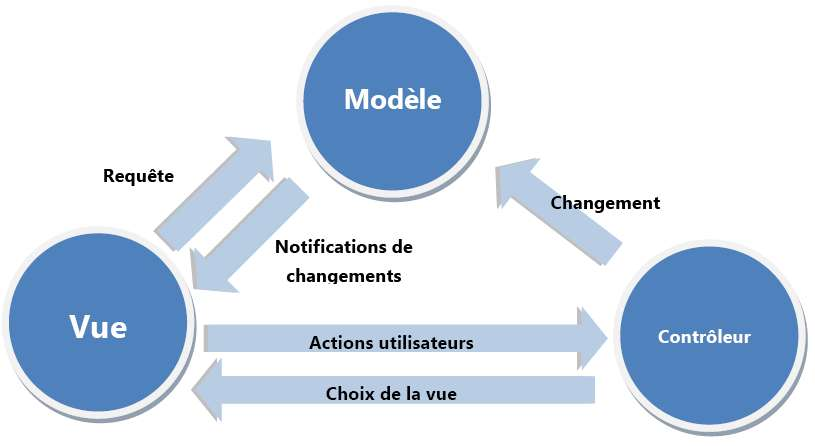
\includegraphics[scale=0.4]{img/mvc.jpg} 
			\end{minipage}
			&
			\begin{minipage}{4cm}
			Permet de modifier :
			\begin{itemize} 
				\item Gameplay
				\item Interface graphique
			\end{itemize} 
			\end{minipage}
		\end{tabular}	
	\end{frame}

	\begin{frame}
	\frametitle{Réutilisabilité}
	\framesubtitle{Nouveaux types de parties}

	
	\begin{tabular}{cc}
	\begin{minipage}{5cm}
		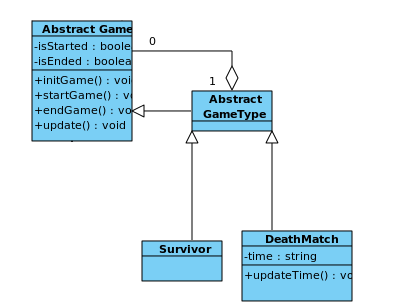
\includegraphics[scale=0.4]{img/decorateur.png} 
	\end{minipage}
	&
	\begin{minipage}{5cm}
	\begin{itemize} 
		\item Design pattern décorateur
		\item Permet l'extension du modèle
	\end{itemize} 
	\end{minipage}
	\end{tabular}
	
	\end{frame}
	

	\begin{frame}
	\frametitle{Réutilisabilité}
	\framesubtitle{Personnalisation}
	
		XML
			L'utilisation du XML permet d'ajouter ou de personnaliser facilement :
			\begin{itemize}
				\item Des objets (bonus, blocs, bombes, etc \ldots)
				\item Des images (themes)
				\item Des sons
			\end{itemize}
	\end{frame}
	

\subsection{Serveur}

	\begin{frame}
	\frametitle{Réutilisabilité}
	\framesubtitle{Fonctionnalités}
	
		\begin{itemize}
			\item Nouvelles servlets = nouvelles fonctionnalités
			\item Même hiérarchie de classes que du côté client 
		\end{itemize}
		
	\end{frame}